% Baza danych
\chapter{Baza danych}

W projekcie została wykorzystana baza danych Firebase Firestore, która jest rozwiązaniem typu NoSQL, opierającym się na dokumentach. Przez Firebase oferowana jest również baza Realtime Database, jednak po dokładnym rozważeniu różnic pomiędzy nimi zdecydowano się ją odrzucić. Głównym przeznaczeniem Realtime Database jest bowiem, jak sugeruje nazwa, przechowywanie i praca na szybko zmieniających się danych, dla których zapewnia małe opóźnienia i wydajną synchronizację pomiędzy klientami. Może to mieć duże znaczenie w przypadku gier, lecz dla tworzonych aplikacji nie jest to krytyczny aspekt. Baza Firestore oferuje za to bardziej intuicyjny sposób przechowywania danych, szybsze oraz bardziej złożone zapytania oraz lepszą skalowalność.

Sposób przechowywania danych przez bazę Firestore w znaczny sposób odbiega od sposobu robienia tego w klasycznych bazach relacyjnych. Zapisuje ona wszystkie dane w dokumentach, które są pogrupowane w kolekcje. Poza istnieniem wysokopoziomowych kolekcji możliwe jest również tworzenie podkolekcji wewnątrz dokumentów, przez co można osiągnąć zagnieżdżoną strukturę.

% Zarówno dokumenty jak i kolekcje posiadają identyfikatory.

\section{Model bazy danych}

Firestore, jako nierelacyjna baza danych, nie posiada modelu, czy schematu, a przynajmniej nie jest on narzucony przez samą bazę. Objawia się to tym, że pozwala ona na przechowywanie wewnątrz jednej kolekcji dokumentów posiadających kompletnie różne zestawy pól, a nawet dynamiczną zmianę ich typów. Mimo wszystko, baza wymaga pewnego uporządkowania i podczas jej projektowania wykształcił się pewien schemat, który zostanie opisany.

Na rysunku \ref{fig:baza-kolekcje} przedstawione zostały wykorzystane kolekcje. Jak widać przewidzianych zostało osiem wysokopoziomowych kolekcji oraz trzy podkolekcje. Należy je rozumieć w taki sposób, że każdy jeden dokument wewnątrz kolekcji \code{offers} posiada własną kolekcję \code{messages}, a każdy jeden dokument wewnątrz kolekcji \code{clients} oraz \code{experts} posiada własną kolekcję \code{tokens}. 

\begin{figure}[ht]
  \centering
  \includegraphics[width=\linewidth]{images/db_collections.png}
  \caption{Diagram stworzonych w bazie kolekcji}
  \label{fig:baza-kolekcje}
\end{figure}

\vspace{\baselineskip}

% \noindent Znaczenie stworzonych kolekcji jest następujące:
\noindent W każdej kolekcji przechowywane są dokumenty reprezentujące inne obiekty, które są następujące:
\begin{itemize}
    \item \textbf{\code{services}} - usługi, które klienci mogą zlecać, a wykonawcy wykonywać;
    \item \textbf{\code{categories}} - kategorie, na które zostały podzielone usługi;
    \item \textbf{\code{clients}} - klienci;
    \item \textbf{\code{experts}} - wykonawcy;
    \item \textbf{\code{jobs}} - zlecenia tworzone przez klientów;
    \item \textbf{\code{offers}} - oferty zgłaszane do zleceń;
    \item \textbf{\code{ratings}} - oceny dawane wykonawcom przez klientów;
    \item \textbf{\code{matches}} - informacje o wykonawcach dopasowanych do zleceń;
    \item \textbf{\code{tokens}} - tokeny FCM, wykorzystywane do wysyłania notyfikacji;
    \item \textbf{\code{messages}} - wiadomości wysyłane przez chat.
\end{itemize}

\vspace{\baselineskip}

Dokładna zawartość dokumentów znajdujących się w wymienionych kolekcjach została przedstawiona na rysunku \ref{fig:baza-dokumenty}. Wraz z każdym znajdującym się w nich polem wypisane zostały typy, które może ono przyjmować. Dla oznaczenia, że dane pole może być nieobecne wprowadzono sztuczny typ \code{absent}, który to oznacza.

\begin{figure}[ht!]
  \centering
  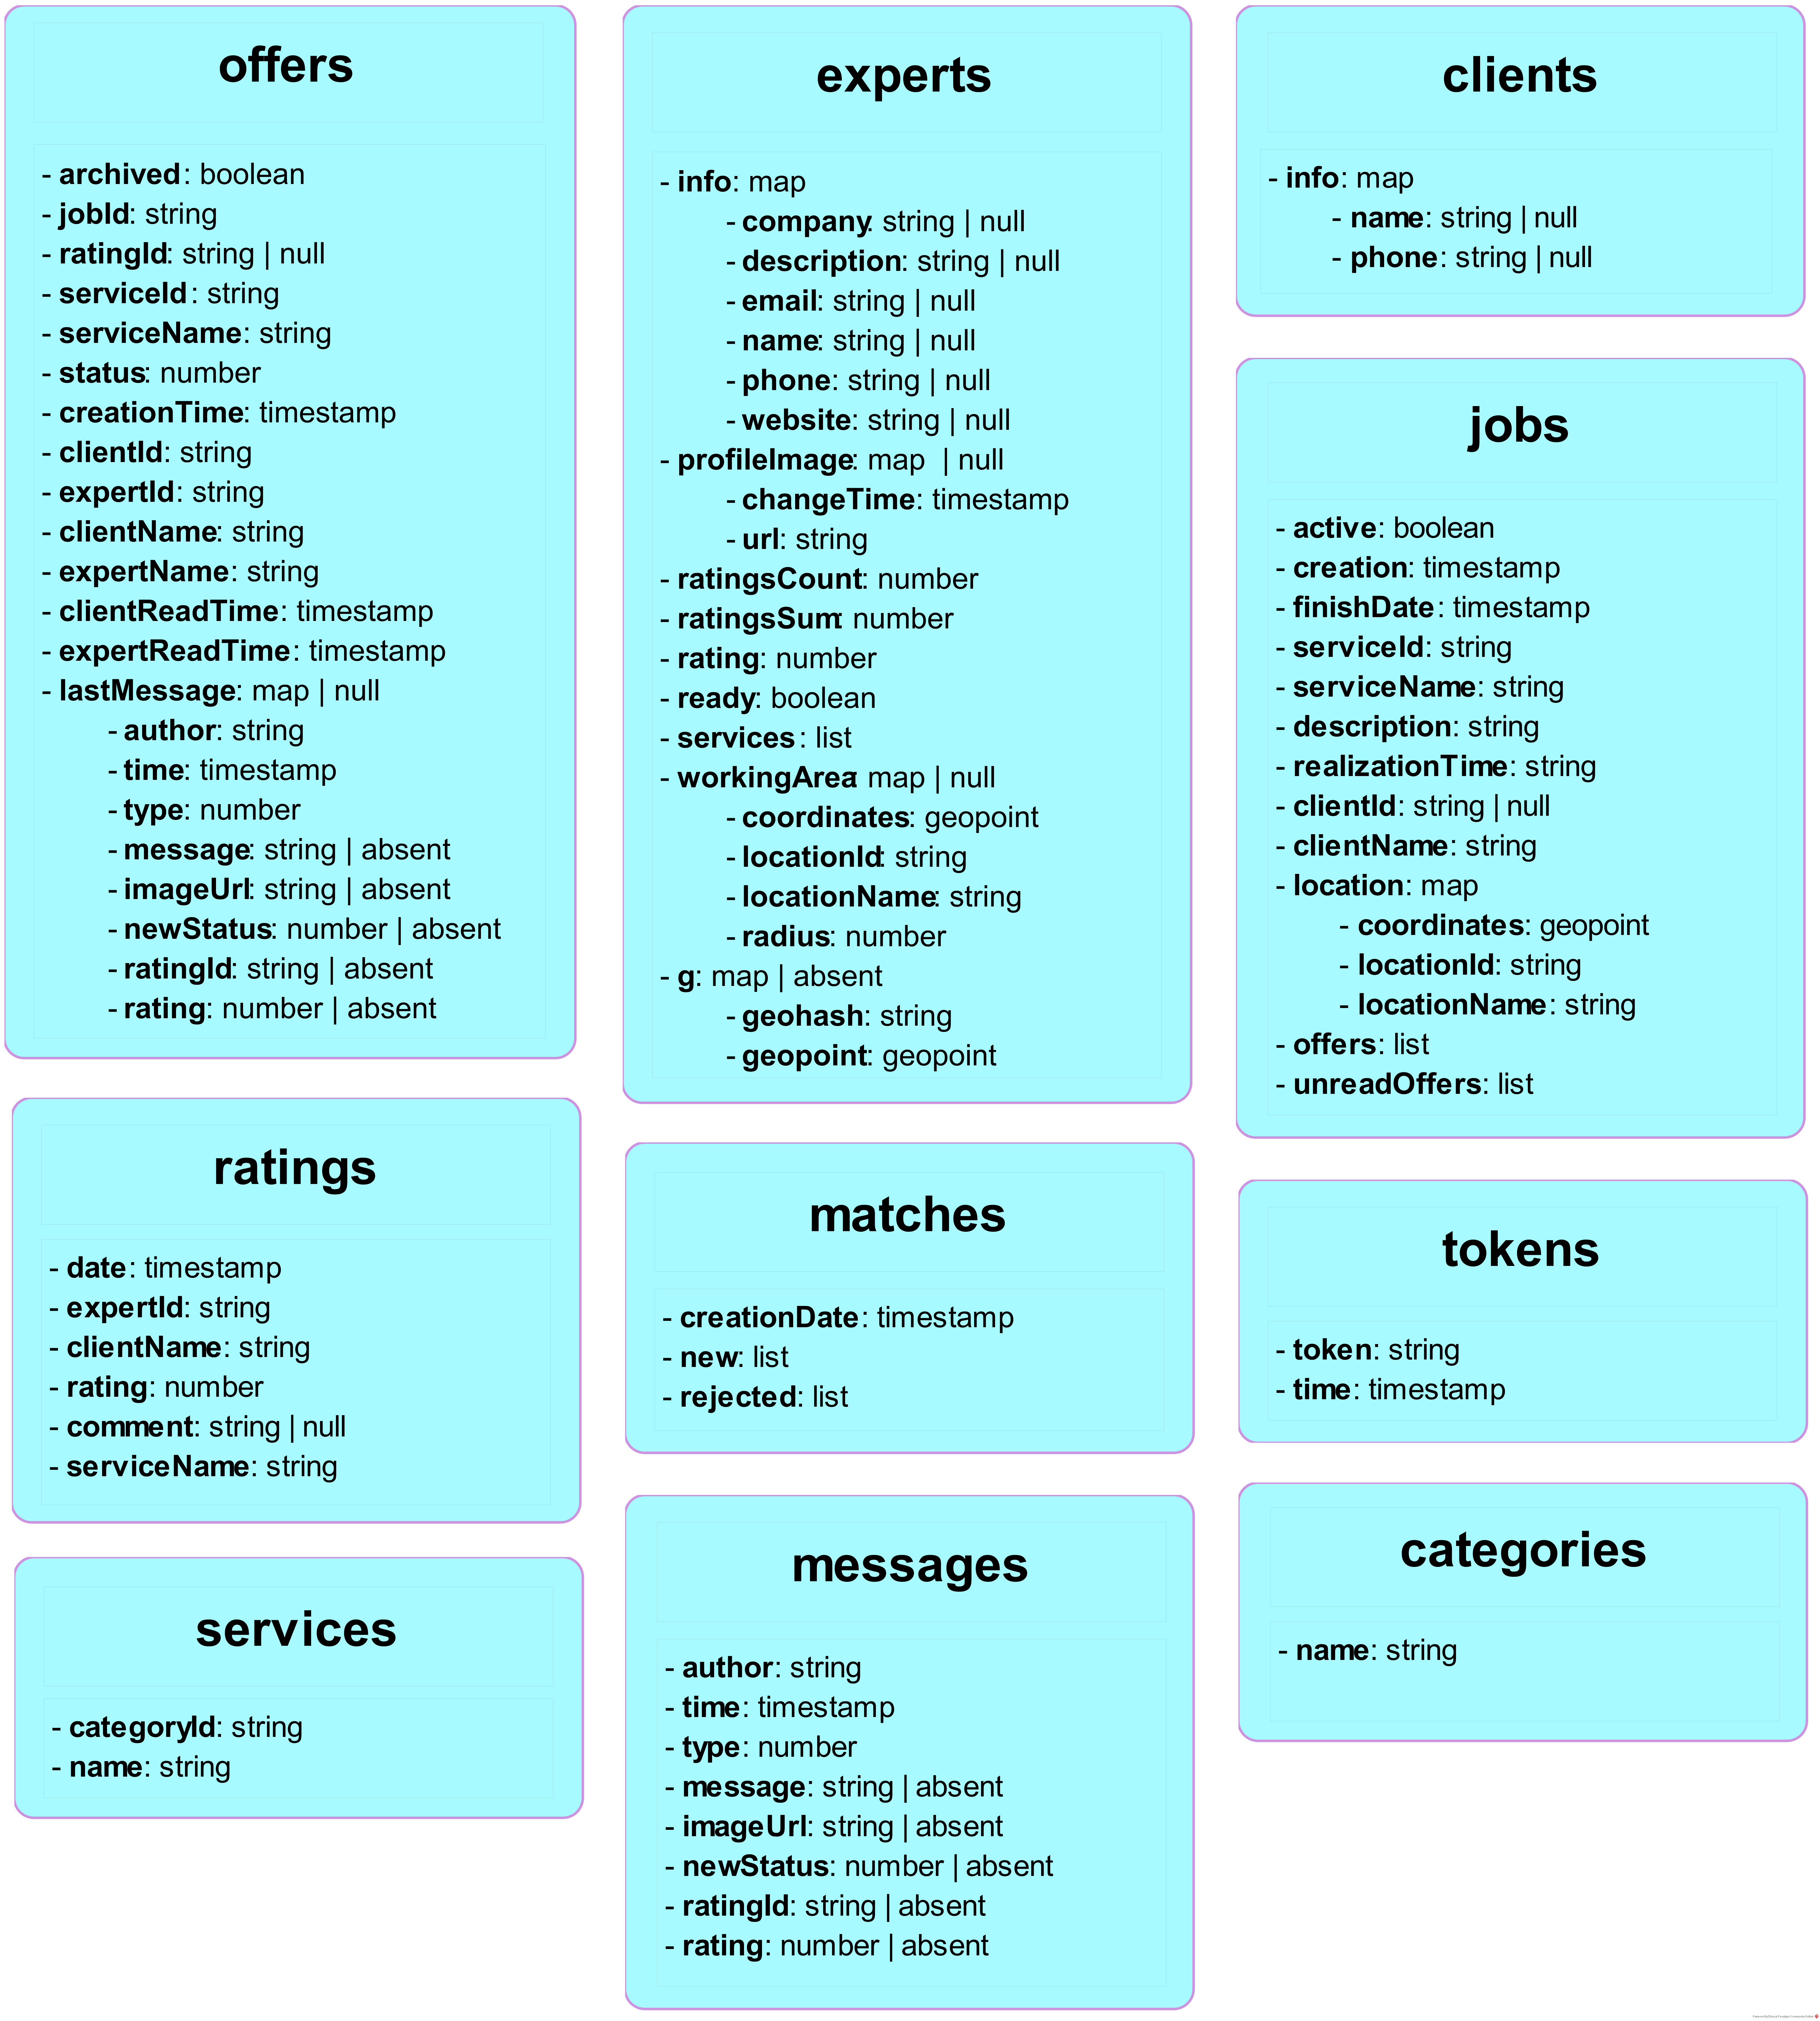
\includegraphics[width=\linewidth]{images/db_documents.png}
  \caption{Schematy dokumentów w poszczególnych kolekcji bazy danych}
  \label{fig:baza-dokumenty}
\end{figure}

\pagebreak

Łączenie pomiędzy dokumentami dokonuje się poprzez umieszczenie w jednym z nich identyfikatora innego. Przykładem tego jest znajdujące się wewnątrz dokumentów w kolekcji \code{services} pole \code{categoryId}, które zawiera identyfikator dokumentu z kolekcji \code{categories} i w ten sposób stworzona zostaje jednokierunkowa relacja jeden do wielu pomiędzy usługami, a ich kategoriami. Nadając nazwy pól przyjęto konwencję, że każde pole, którego nazwa posiada sufiks \code{Id} jest referencją do innego dokumentu.

\section{Redundancja}

\noindent Redundancja to nadmiarowość w stosunku do tego, co konieczne. W przypadku baz danych jej prostym przykładem jest przechowywanie tych samych informacji w kilku miejscach. Zwykle dąży się do usunięcia redundancji, czyli normalizacji, ponieważ niepotrzebnie zwiększa rozmiar bazy i naraża ją na brak spójności. Mimo wszystko można ją zaobserwować na przedstawionym schemacie bazy w następujących miejscach:

% \noindent Na szczególną uwagę zasługuję istniejąca w bazie w kilku miejscach redundancja. Jest 

\vspace{0.5\baselineskip}

\begin{itemize}
    \item Dokumenty w kolekcjach \code{offers} oraz \code{jobs} posiadają pole \code{serviceName} zawierające nazwę usługi, chociaż wartość ta może zostać uzyskana poprzez wykorzystanie referencji \code{serviceId}, znajdującej się w tych dokumentach i odczytanie pola \code{name} z odpowiedniego dokumentu w kolekcji \code{services}.
    \item Dokumenty w kolekcji \code{offers} posiadają pole \code{expertName} zawierające imię i nazwisko wykonawcy, chociaż wartość ta może zostać uzyskana poprzez wykorzystanie referencji \code{expertId}, znajdującej się w tych dokumentach i odczytanie pola \code{info.name} z odpowiedniego dokumentu w kolekcji \code{experts}.
    \item Dokumenty wewnątrz kolekcji \code{offers} oraz \code{jobs} posiadają pole \code{clientName} zawierające imię i nazwisko klienta, chociaż wartość ta może zostać uzyskana poprzez wykorzystanie referencji \code{clientId}, znajdującej się w tych dokumentach i odczytanie pola \code{info.name} z odpowiedniego dokumentu w kolekcji \code{clients}.
\end{itemize}

Wskazana redundancja została wprowadzona celowo, a jej przeznaczeniem jest uniknięcie konieczności podążania referencjami i odczytywania dodatkowych dokumentów. Generowałoby to dodatkowe koszty, ponieważ Firebase nalicza je między innymi względem liczby odczytanych dokumentów. Dodatkowo przyczyniłoby się do większego ruchu sieciowego, który na urządzeniach mobilnych należy ograniczać z powodu zużycia baterii i możliwych ograniczeń transferu.

Aby zrozumieć, dlaczego redundancja została wprowadzona akurat w tych miejscach należy odwołać się do interfejsu użytkownika, a konkretnie ekranów przedstawionych na rysunku \ref{fig:ekrany-redundancja}. Są to główne ekrany obu aplikacji, więc będą często wyświetlane i wszystkie trzy zawierają listy, które mogą być potencjalnie bardzo długie. Są więc ekranami w przypadku których szczególnie warto zadbać o minimalizację liczby odczytywanych dokumentów. 

\begin{figure}[ht]
  \captionsetup[subfigure]{justification=centering}
  \centering
  \begin{subfigure}{0.32\textwidth}
    \centering
    \fbox{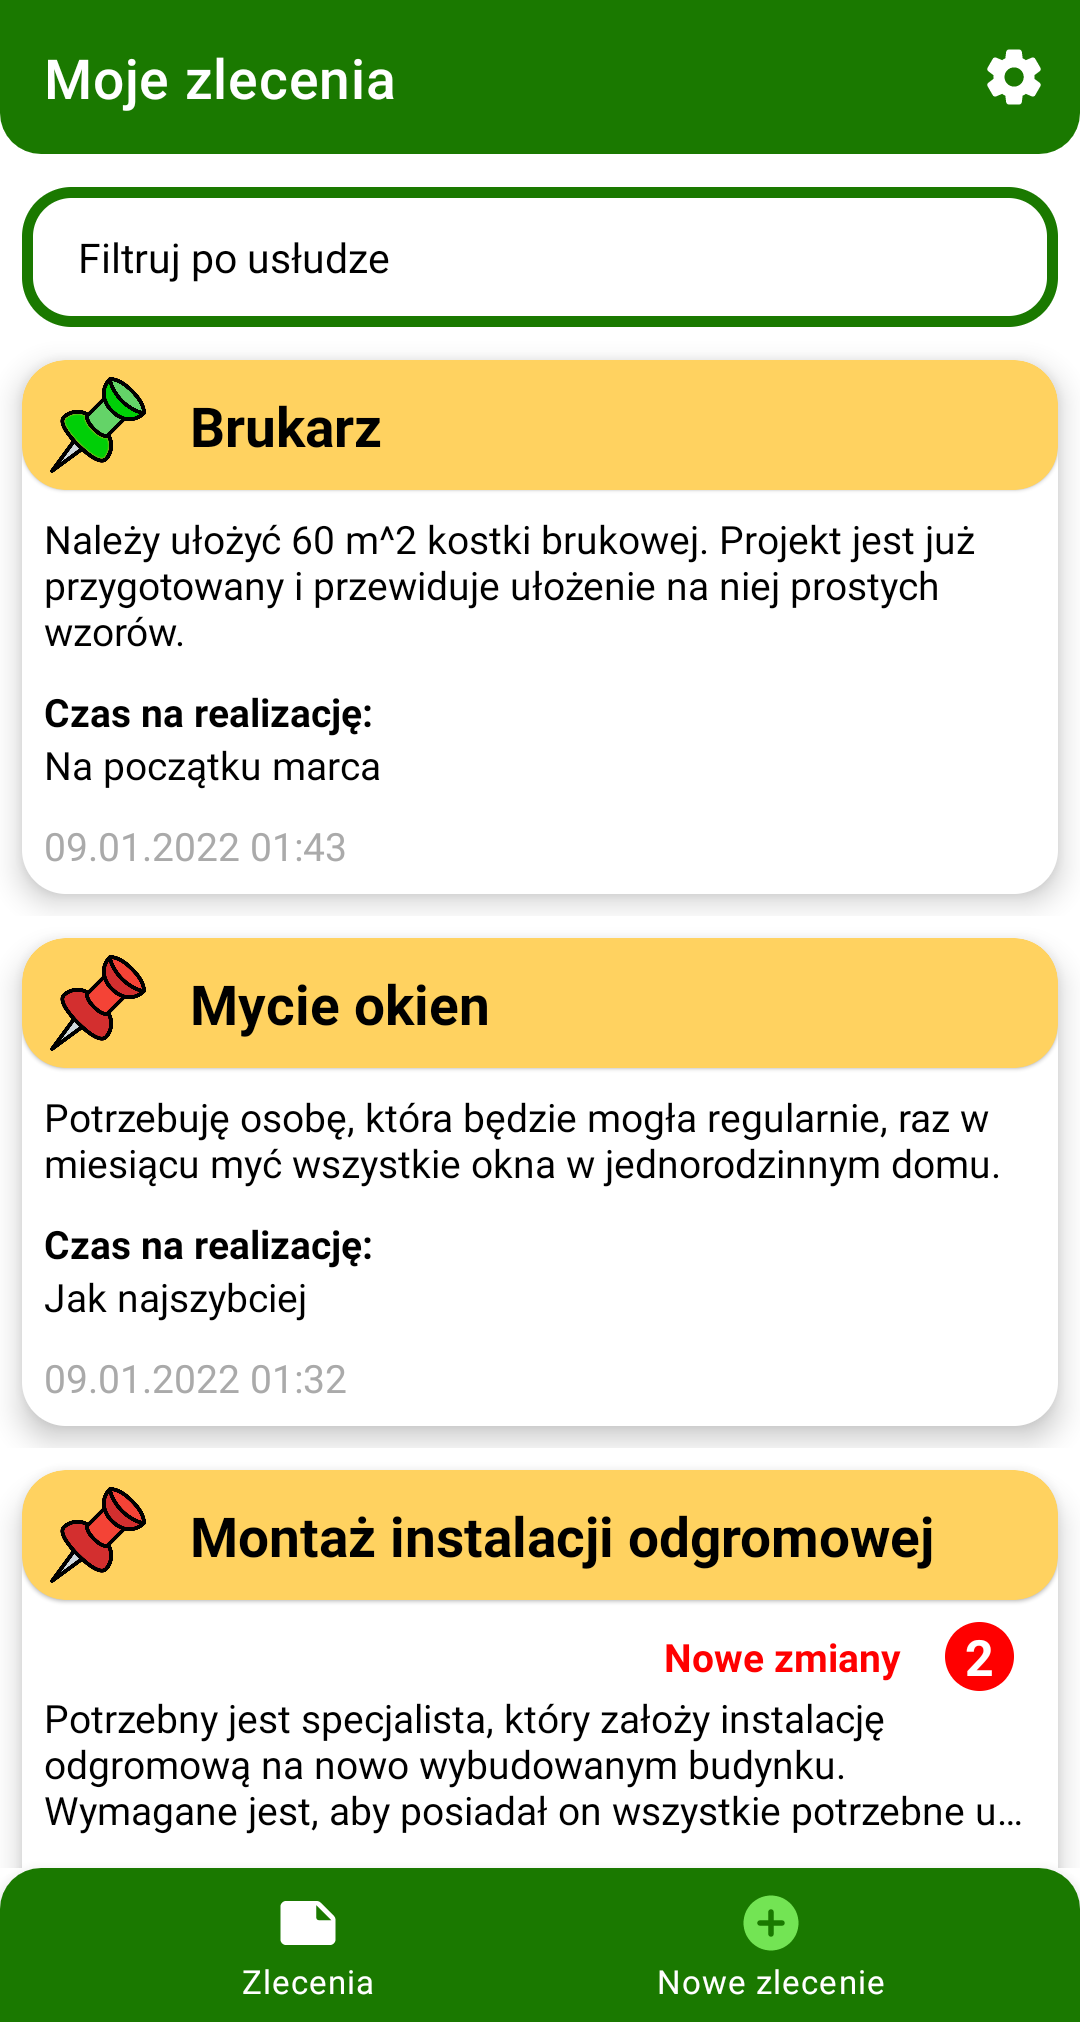
\includegraphics[width=0.97\linewidth]{screens/client_jobs.png}}
    \caption{Ekran dodanych zleceń\\(aplikacja dla klientów)}
  \end{subfigure}
  \begin{subfigure}{0.32\textwidth}
    \centering
    \fbox{
\includegraphics[width=0.95\linewidth]{screens/expert_jobs.png}}
    \caption{Ekran dostępnych zleceń\\(aplikacja dla wykonawców)}
  \end{subfigure}
  \begin{subfigure}{0.32\textwidth}
    \centering
    \fbox{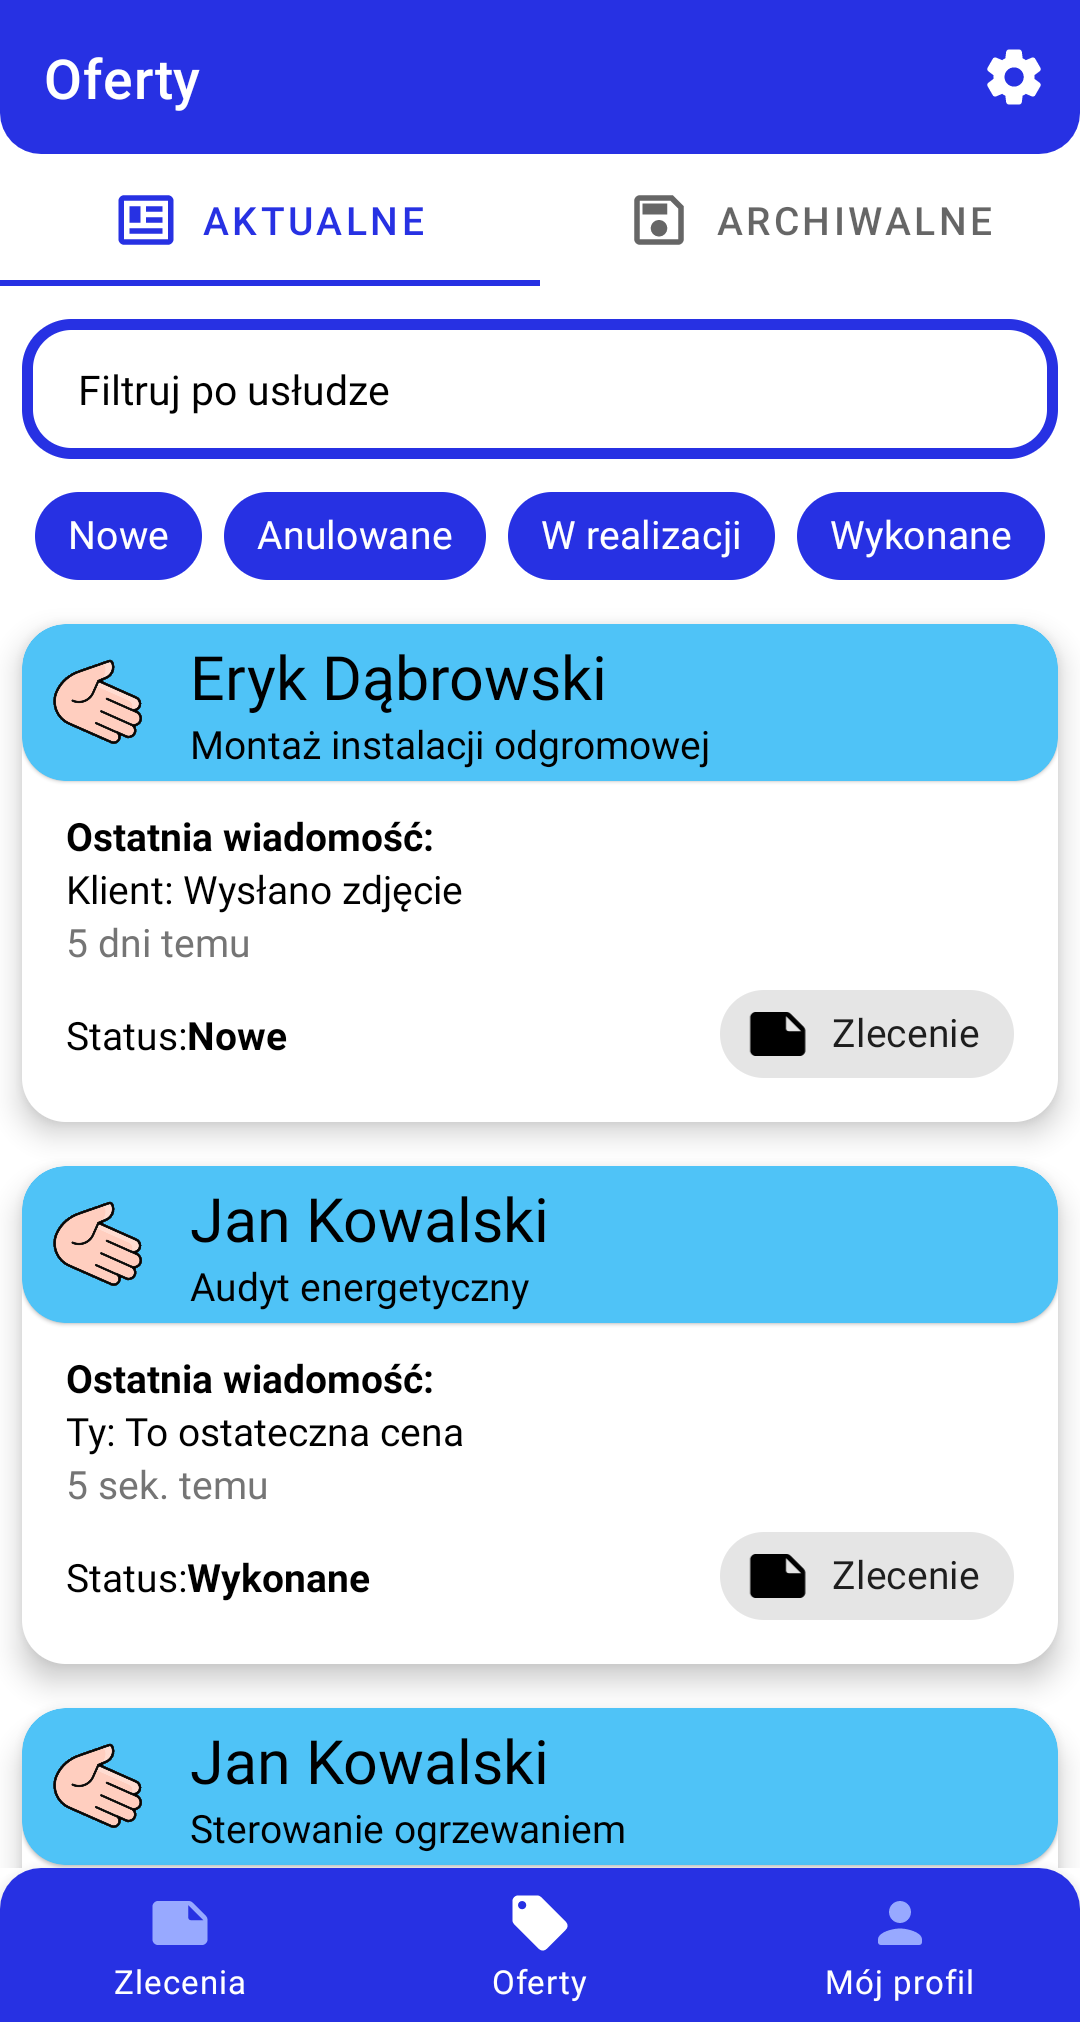
\includegraphics[width=0.95\linewidth]{screens/expert_offers_no_swap.png}}
    \caption{Ekran złożonych ofert\\(aplikacja dla wykonawców)}
  \end{subfigure}
  \caption{Ekrany mające wpływ na wprowadzoną w bazie redundancję}
  \label{fig:ekrany-redundancja}
\end{figure}

W przypadku ekranu (a), przedstawionego na rysunku \ref{fig:ekrany-redundancja}, lista zawiera zlecenia, wraz z nazwami usług, których dotyczą. Dzięki temu, że dokumenty zleceń zawierają nazwy usług, to dla każdego elementu listy wystarczy odczytać tylko jeden dokument. W przeciwnym wypadku konieczne byłoby zaangażowanie dodatkowej kolekcji i zwiększenie liczby odczytywanych dokumentów dwukrotnie.

W przypadku ekranu (b) dla każdego zlecenia, oprócz nazwy usługi, wyświetlana jest również nazwa klienta, więc w tym przypadku redundancja pozwala zmniejszyć liczbę odczytywanych dokumentów nawet trzykrotnie.

Dla ekranu (c) redundancja również zmniejsza liczbę odczytywanych dokumentów trzykrotnie, ponieważ umożliwia uniknięcie odczytywania dokumentów z kolekcji \code{experts}, by dostać nazwisko wykonawcy i kolekcji \code{services}, by dostać nazwę usługi.

% Należy zauważyć, że aby wprowadzanie redundancji było sensowne to częstotliwość odczytywania rozważanych informacji musi być znacząco większa od częstotliwości ich modyfikacji, ponieważ konieczne jest utrzymywanie spójności danych, poprzez aktualizowanie wartości we wszystkich miejsach na raz, zamiast jednego

\section{Zapytania związane z lokalizacjami}

Baza danych, wśród innych informacji, przechowuje lokalizacje związane ze zleceniami oraz wykonawcami. Jest to bardzo proste z powodu dostępnego w Firestore typu geopoint, zawierającego w sobie zarówno szerokość, jak i wysokość geograficzną. Okazuje się jednak, że pomimo obecności tego typu, baza nie wspiera wykonywania żadnych specyficznych dla lokalizacji kwerend. 
Podczas implementacji okazało się jednak konieczne zwrócenie wszystkich dokumentów zawierających lokalizację, znajdującą się w zadanym maksymalnym promieniu od pewnego, centralnego punktu. Operacja ta została zwizualizowana na rysunku \ref{fig:query}.

\begin{figure}[ht]
  \centering
  \fbox{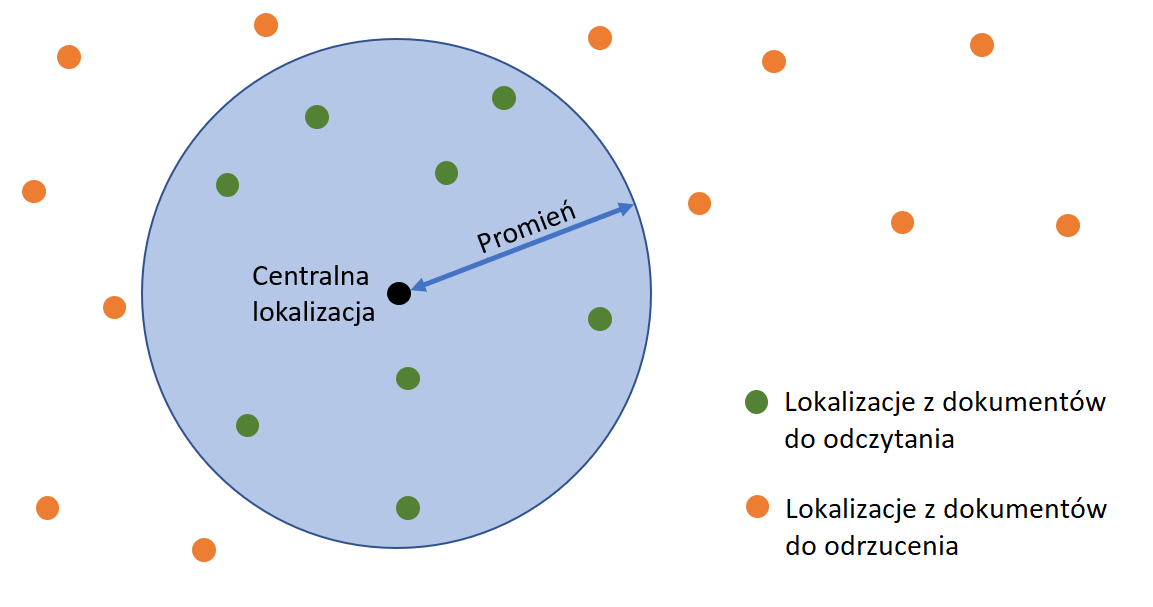
\includegraphics[width=0.7\linewidth]{images/query_visualization.png}}
  \caption{Wizualizacja potrzebnej operacji związanej z lokalizacją}
  \label{fig:query}
\end{figure}

Jak zostało wspomniane, Firestore nie posiada żadnych mechanizmów ułatwiających wykonanie tego typu zapytania. Wciąż istnieją jednak pewne drogi umożliwiające rozwiązanie powstałego problemu.

Najbardziej naiwnym rozwiązaniem jest pobieranie wszystkich dokumentów jeden po drugim, obliczanie dla każdego z nich odległości do centralnej lokalizacji i zaliczanie do zbioru wynikowego, jeżeli jest ona odpowiednio mała. Ma to jednak ogromną wadę w postaci odczytu dużej liczby dokumentów i w związku z tym generowaniem wysokich kosztów. Z tego powodu metoda ta została szybko odrzucona.

Rozsądnym rozwiązaniem byłoby określenie ramki okalającej (ang. bounding box), w której muszą znajdować się wszystkie lokalizacje z potrzebnych do odczytania dokumentów. Mogłyby z niej zostać odczytane poprzez dokonanie filtracji jednocześnie po odpowiednim zakresie szerokości i wysokości geograficznych. Problem w tym, że Firestore nie pozwala na wykonanie takiej operacji w jednym zapytaniu. W jednej kwerendzie należałoby dokonać filtracji po zakresie szerokości, a w drugiej po zakresie wysokości i przeprowadzić ręczne połączenie ich wyników operacją iloczynu mnogościowego. Podczas niej zostanie jednak odrzuconych wiele dokumentów, co oznacza, że ich odczyty spowodowały niepotrzebne koszty.

% Rozsądnym podejściem byłoby zwrócenie nieco większego zbioru dokumentów poprzez dokonanie filtracji jednocześnie po odpowiednim zakresie szerokości i wysokości geograficznych, a następnie odrzucenie z niego niechcianych elementów. Problem w tym, że Firestore nie pozwala wykonania takiej operacji w jednym zapytaniu. Konieczne byłoby wykonanie dwóch kwerend, a następnie samodzielne połączenie ich wyniku. Również ta metoda wiąże się z dużą liczbą niepotrzebnie odczytywanych dokumentów.

% Najlepszym rozwiązaniem okazuje się wykorzystanie geohashy, które umożliwiają wydajne wykonywanie tego typu operacji. Są one ciągami znaków, w których zakodowana jest zarówno szerokość, jak i wysokość geograficzna. Mają ciekawą własność polegającą na tym, że im wspólny prefiks dwóch z nich jest dłuższy, tym lokalizacje, które reprezentują, znajdują się bliżej siebie. Geohashe zostały dodane do dokumentów z kolekcji \code{experts}. Aby zapewnić możliwość prostego ich wykorzystania, została użyta biblioteka geofirestore. Zapewnia ona wyszukiwanie dokumentów na podstawie położenia geograficznego i dostarcza potrzebną operację.

Najlepszym rozwiązaniem okazuje się wykorzystanie geohashy, które umożliwiają wydajne wyszukiwanie na podstawie lokalizacji. Są one ciągami znaków, w których zakodowana jest zarówno szerokość, jak i wysokość geograficzna. Mają ciekawą właściwość polegającą na tym, że im wspólny prefiks dwóch z nich jest dłuższy, tym lokalizacje, które reprezentują, znajdują się bliżej siebie. Aby zapewnić możliwość ich prostego wykorzystania, została użyta biblioteka geofirestore. Zapewnia ona wyszukiwanie dokumentów na podstawie położenia geograficznego i dostarcza potrzebną operację.

% \begin{figure}[ht]
%   \centering
%   \includegraphics[width=0.5\linewidth]{images/geohash_fancy.png}
%   \caption{Wizualizacja logiki stojącej za algorytmem geohashy \cite{geohash-fancy}}
%   \label{fig:geohash}
% \end{figure}